\documentclass[a4paper,11pt]{article}
\usepackage{fontspec}
\usepackage[french]{babel}
\usepackage{geometry}
\usepackage{graphicx}
\usepackage{titlesec}
\PassOptionsToPackage{hyphens}{url}\usepackage{hyperref}
\usepackage{setspace}
\usepackage{svg}
\usepackage{newtxmath}
\usepackage{float}
\usepackage{minted}
% to display code
\usepackage{listings}
\usepackage{xcolor}
\definecolor{bggray}{rgb}{0.90,0.90,0.90}
\definecolor{bggraylight}{rgb}{0.95,0.95,0.95}
% Customize the appearance of inline code
\setmintedinline{
    bgcolor=bggray,
    fontsize=\footnotesize,
    breaklines=true
    }

\setminted{
    bgcolor=bggraylight,
    breaklines=true,
    frame=lines,
    mathescape,
    autogobble=true,
    breakanywhere=true,
    breakautoindent=true,
    fontsize=\footnotesize
}

\setmainfont{Montserrat}
\setmonofont{JetBrains Mono}

% Marges
\geometry{margin=1in}

% Interligne de 1.5
\setstretch{1.5}

% Titres en gras et numérotés
\titleformat{\section}{\bfseries\Large}{\thesection}{1em}{}
\titleformat{\subsection}{\bfseries\large}{\thesubsection}{1em}{}

% Commande pour un titre centré
\newcommand{\reporttitle}[1]{%
  \begin{center}
    \LARGE\textbf{#1}
  \end{center}
  \vspace{1cm}
}
% Début du document
\begin{document}

% Page de garde
\begin{titlepage}
    \begin{center}
        \vspace*{2cm}
        \Huge\textbf{Database reverse engineering and assessment for
            Android applications}\\
        \vspace{1cm}
        \Large INFOM218 - Année académique 2024-2025\\
        \begin{figure}[!ht]
            \centering
            
\includegraphics[scale=0.1]{images/vespucci.png}
            \label{fig:logo-vespucci}
        \end{figure}
        {\Large\textbf{Groupe 1}}\\
        \vspace{0.5cm}
        {\Large François Bechet\\
            Thibaut Berg}\\
        Anaé De Baets\\
        Carine Pochet\\
        \vspace{1cm}
        {\Large\textbf{Professeur}}\\
        \vspace{0.5cm}
        {\Large Prof. Anthony Cleve}\\
        \vfill
        \begin{figure}[!ht]
            \centering
            \includesvg[width=0.2\textwidth]{images/logo_unamur}
            \label{fig:logo-unamur}
        \end{figure}
        \Large Université de Namur\\
        \Large \today
    \end{center}
\end{titlepage}

% Table des matières
\tableofcontents
\newpage

% Contenu du rapport
\section{Partie 1}
\subsection{Schéma physique}
Pour extraire les données du schéma physique, nous avons utilisé le plugin SQLInspect sur Eclipse afin de récupérer toutes les requêtes SQL du programme. Un script python a ensuite été créé afin de pouvoir trier les différentes requêtes en fonction de mots-clefs. La combinaison des différentes requêtes de création des tables ainsi que des contrainte a mené à ce résultat. On peut y retrouver 6 clefs étrangères qui ne référencent pas toujours des champs uniques. La seule clef primaire composée est située sur la table « tiles ». On retrouve une multitude de champs qui sont nullable. Ces derniers peuvent être utilisés comme référence dans une clef étrangère.
Toutes les tables présentent des noms qui sont plutôt explicites. On comprend son utilité et les données qui y sont stockées. Il en va de même pour la majorité des noms d'attributs.
\begin{figure}[h!]
    \centering
    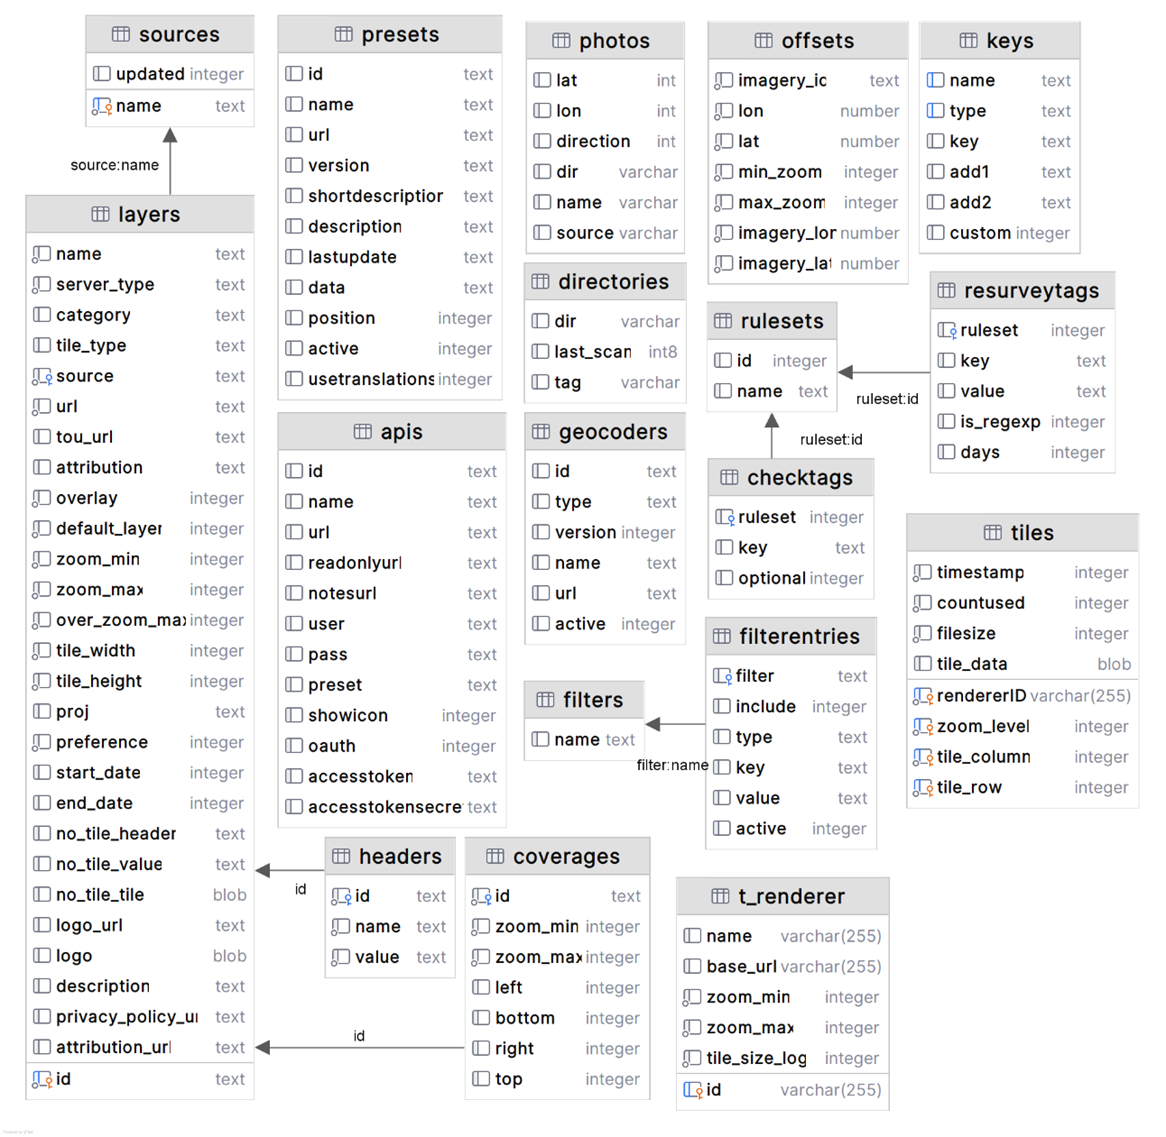
\includegraphics[scale=1]{schema_physique.png}
    \label{fig:schéma physique}
\end{figure}

\subsection{Analyse supplémentaire pour découvrir des Foreign Keys}
\subsubsection{Recherche dans le code source}
Aucune clef étrangère implicite n'a été trouvée suite à l'analyse des requêtes SELECT avec la regex : « (FROM|from).*,.*(WHERE|where)». Cette dernière permet de sélectionner les requêtes qui réalisent un SELECT sur plusieurs tables.
Une seconde analyse des requêtes n'a donné aucun résultat pour le format de jointure SQL2. Une simple recherche du mot clef « JOIN » ne donne aucun résultat, autant dans les requêtes listées par SQLInspect ni dans le code source de l'application.

\subsubsection{Recherche de patterns}
Les tables « directories » et « photos » ont toutes les 2 un attribut « dir ». En analysant le code du fichier « PhotoIndex.java », et plus précisément de la méthode « private void indexDirectories() », on remarque qu'une query sur la table « photos » utilise la valeur de l'attribut « dir » récupéré à partir d'un select sur la table « directories ». Il y a donc un lien implicite entre ces 2 tables. Toutefois la requête utilise le mot clef « LIKE » qui permet de récupérer les entrés où l'attribut « dir » de la table « photos » contient l'attribut « dire » de la table « directories » suivi ou non d'autres caractères (symbolisé par « \% » dans la requête).

\subsection{Schéma logique}

\subsection{Schéma conceptuel}

\begin{figure}[h!]
    \centering
    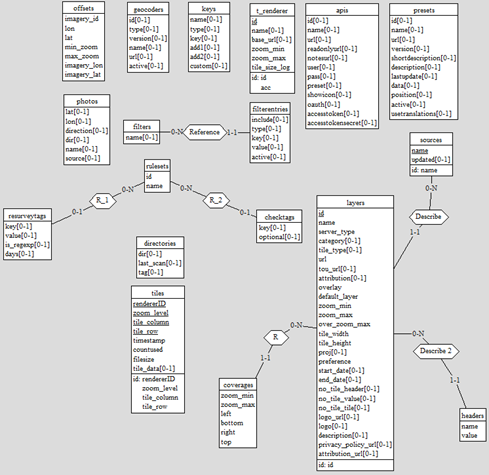
\includegraphics[scale=1]{schema_conceptuel.png}
    \label{fig:schéma conceptuel}
\end{figure}
\newpage
\section{Partie 2}

\subsection{Statistiques}

\begin{table}[H]
    \centering
    \begin{tabular}{|l|c|c|}
        \hline
        \textbf{Type}  & \textbf{\# trouvées par SOLInspect} & \textbf{\# trouvées manuellement} \\ \hline
        SELECT         & 18                                  & 24                                \\ \hline
        UPDATE         & 4                                   & 24                                \\ \hline
        DELETE         & 2                                   & 27                                \\ \hline
        INSERT         & 5                                   & 16                                \\ \hline
        CREATE TABLE   & 18                                  & 18                                \\ \hline
        CREATE INDEX   & 8                                   & 8                                 \\ \hline
        ALTER TABLE    & 24                                  & 24                                \\ \hline
        \textbf{Total} & \textbf{79}                         & \textbf{141}                      \\ \hline
    \end{tabular}
    \caption{Nombre de requêtes trouvées par type.}
\end{table}

Pour les requêtes de la colonne « \# trouvées manuellement », un script \texttt{Python} a été utilisé pour effectuer une analyse statique des requêtes. Il permet de parcourir les différents fichiers Java et, grâce à une regex, les différents appels à SQLite tels que \mintinline{java}{db.update} ou encore \mintinline{java}{db.execSQL} sont filtrés et enregistrés dans des fichiers séparés.

Pour la complexité de ces dernières, elles sont plutôt simples et courtes. On notera toutefois que les requêtes de création de table peuvent être plus longues, notamment pour la table \mintinline{java}{presets}, mais restent, malgré tout, simples à interpréter.

À propos de la répartition des requêtes dans le projet, elles sont regroupées dans 12 fichiers Java différents. Ces 12 fichiers sont répartis parmi 7 dossiers alors que le projet en compte 58.

\begin{table}[H]
    \centering
    \begin{tabular}{|l|l|}
        \hline
        \textbf{Dossier}                                     & \textbf{Fichier}                           \\ \hline
        \texttt{src/main/java/de/blau/android/filter}        & \texttt{TagFilterActivity.java}            \\
                                                             & \texttt{TagFilterDatabaseHelper.java}      \\ \hline
        \texttt{src/main/java/de/blau/android/imageryoffset} & \texttt{ImageryOffsetDatabase.java}        \\ \hline
        \texttt{src/main/java/de/blau/android/photos}        & \texttt{PhotoIndex.java}                   \\ \hline
        \texttt{src/main/java/de/blau/android/prefs}         & \texttt{AdvancedPrefDatabase.java}         \\ \hline
        \texttt{src/main/java/de/blau/android/resources}     & \texttt{KeyDatabaseHelper.java}            \\
                                                             & \texttt{TileLayerDatabase.java}            \\ \hline
        \texttt{src/main/java/de/blau/android/services/util} & \texttt{MapTileProviderDataBase.java}      \\
                                                             & \texttt{MBTileProviderDataBase.java}       \\ \hline
        \texttt{src/main/java/de/blau/android/validation}    & \texttt{ValidatorRulesDatabase.java}       \\
                                                             & \texttt{ValidatorRulesDatabaseHelper.java} \\
                                                             & \texttt{ValidatorRulesUI.java}             \\ \hline
    \end{tabular}
    \caption{Répartition des fichiers contenant des requêtes SQL.}
\end{table}

\newpage
\section{Partie 3}
\subsection{Scénario d'évolution n°1}

\subsubsection{Scénario}
Renommer la colonne \mintinline{java}{name} de la table \mintinline{java}{headers}.
\subsubsection{Modifications}
Pour renommer la colonne \mintinline{java}{name} de la table \mintinline{java}{headers}, les étapes suivantes sont nécessaires. Ces changements concernent le code source et le schéma SQL dans différents fichiers du projet.

\begin{enumerate}
    \item \textbf{Changer la constante qui représente le nom de la colonne}
          \begin{itemize}
              \item \textbf{Fichier concerné} : \texttt{TileLayerDatabase.java}
              \item \textbf{Emplacement} : \href{https://github.com/MarcusWolschon/osmeditor4android/blob/dcabe8084aa15f5551a37c990516bf73398af1bf/src/main/java/de/blau/android/resources/TileLayerDatabase.java#L82}{Ligne 82}
              \item \textbf{Ancien code} :
                    \begin{minted}{java}
                        private static final String HEADER_NAME_FIELD = "name";
                    \end{minted}
              \item \textbf{Nouveau code} :
                    \begin{minted}{java}
                        private static final String HEADER_NAME_FIELD = "newName";
                    \end{minted}
          \end{itemize}

    \item \textbf{Modifier la définition de la table dans la méthode \texttt{createHeadersTable}}
          \begin{itemize}
              \item \textbf{Fichier concerné} : \texttt{TileLayerDatabase.java}
              \item \textbf{Emplacement} : \href{https://github.com/MarcusWolschon/osmeditor4android/blob/dcabe8084aa15f5551a37c990516bf73398af1bf/src/main/java/de/blau/android/resources/TileLayerDatabase.java#L161}{Ligne 161}
              \item \textbf{Ancien code} :
                    \begin{minted}{java}
                        private void createHeadersTable(SQLiteDatabase db) {
                            db.execSQL("CREATE TABLE headers (id TEXT NOT NULL, name TEXT NOT NULL, value TEXT NOT NULL,"
                                    + " FOREIGN KEY(id) REFERENCES layers(id) ON DELETE CASCADE)");
                            db.execSQL("CREATE INDEX headers_idx ON headers(id)");
                        }
                    \end{minted}
              \item \textbf{Nouveau code} :
                    \begin{minted}{java}
                        private void createHeadersTable(SQLiteDatabase db) {
                            db.execSQL("CREATE TABLE headers (id TEXT NOT NULL, newName TEXT NOT NULL, value TEXT NOT NULL,"
                                    + " FOREIGN KEY(id) REFERENCES layers(id) ON DELETE CASCADE)");
                            db.execSQL("CREATE INDEX headers_idx ON headers(id)");
                        }
                    \end{minted}
          \end{itemize}

    \item \textbf{Mettre à jour la méthode \texttt{getHeadersById} pour refléter le changement}
          \begin{itemize}
              \item \textbf{Fichier concerné} : \texttt{TileLayerDatabase.java}
              \item \textbf{Emplacement} : \href{https://github.com/MarcusWolschon/osmeditor4android/blob/dcabe8084aa15f5551a37c990516bf73398af1bf/src/main/java/de/blau/android/resources/TileLayerDatabase.java#L716}{Ligne 716}
              \item \textbf{Ancien code} :
                    \begin{minted}{java}
                        @NonNull
                        private static Map<String, List<Header>> getHeadersById(SQLiteDatabase db, boolean overlay) {
                            Map<String, List<Header>> headersById = new HashMap<>();
                            try (Cursor headerCursor = db.rawQuery(
                                    "SELECT headers.id as id,headers.name as name,value FROM layers,headers WHERE headers.id=layers.id AND overlay=?",
                                    new String[] { boolean2intString(overlay) })) {
                                if (headerCursor.getCount() >= 1) {
                                    initHeaderFieldIndices(headerCursor);
                                    boolean haveEntry = headerCursor.moveToFirst();
                                    while (haveEntry) {
                                        String id = headerCursor.getString(headerIdFieldIndex);
                                        List<Header> headers = headersById.get(id);
                                        if (headers == null) {
                                            headers = new ArrayList<>();
                                            headersById.put(id, headers);
                                        }
                                        headers.add(getHeaderFromCursor(headerCursor));
                                        haveEntry = headerCursor.moveToNext();
                                    }
                                }
                            }
                            return headersById;
                        }
                    \end{minted}
              \item \textbf{Nouveau code} :
                    \begin{minted}{java}
                        @NonNull
                        private static Map<String, List<Header>> getHeadersById(SQLiteDatabase db, boolean overlay) {
                            Map<String, List<Header>> headersById = new HashMap<>();
                            try (Cursor headerCursor = db.rawQuery(
                                    "SELECT headers.id as id, headers.newName as newName, value FROM layers, headers WHERE headers.id=layers.id AND overlay=?",
                                    new String[] { boolean2intString(overlay) })) {
                                if (headerCursor.getCount() >= 1) {
                                    initHeaderFieldIndices(headerCursor);
                                    boolean haveEntry = headerCursor.moveToFirst();
                                    while (haveEntry) {
                                        String id = headerCursor.getString(headerIdFieldIndex);
                                        List<Header> headers = headersById.get(id);
                                        if (headers == null) {
                                            headers = new ArrayList<>();
                                            headersById.put(id, headers);
                                        }
                                        headers.add(getHeaderFromCursor(headerCursor));
                                        haveEntry = headerCursor.moveToNext();
                                    }
                                }
                            }
                            return headersById;
                        }
                    \end{minted}
          \end{itemize}
\end{enumerate}
\subsection{Scénario d'évolution n°2}
\subsubsection{Scénario}
Supprimer la table \mintinline{java}{filters}.
\subsubsection{Modifications}
Tous les schémas sont concernés par cette modification, il faut donc y supprimer la table \mintinline{java}{filters}.

\begin{enumerate}
    \item \textbf{Modifier la méthode \mintinline{java}{onCreate}}
          \begin{itemize}
              \item \textbf{Fichier concerné} : \texttt{TagFilterDatabaseHelper.java}
              \item \textbf{Emplacement} :
                    \href{https://github.com/MarcusWolschon/osmeditor4android/blob/master/src/main/java/de/blau/android/filter/TagFilterDatabaseHelper.java#L30}{Ligne 30}
              \item \textbf{Ancien code} :
                    \begin{minted}{java}
                        @Override
                        public void onCreate(SQLiteDatabase db) {
                            try {
                                db.execSQL("CREATE TABLE filters (name TEXT)");
                                db.execSQL("INSERT INTO filters VALUES ('Default')");
                                db.execSQL(
                                        "CREATE TABLE filterentries (filter TEXT, include INTEGER DEFAULT 0, type TEXT DEFAULT '*', key TEXT DEFAULT '*', value TEXT DEFAULT '*', active INTEGER DEFAULT 0, FOREIGN KEY(filter) REFERENCES filters(name))");
                            } catch (SQLException e) {
                                Log.w(DEBUG_TAG, "Problem creating database", e);
                            }
                        }
                    \end{minted}
              \item \textbf{Nouveau code} :
                    \begin{minted}{java}
                        @Override
                        public void onCreate(SQLiteDatabase db) {
                            try {
                                db.execSQL("CREATE TABLE filters (name TEXT)");
                                db.execSQL("INSERT INTO filters VALUES ('Default')");
                                db.execSQL(
                                        "CREATE TABLE filterentries (filter TEXT, include INTEGER DEFAULT 0, type TEXT DEFAULT '*', key TEXT DEFAULT '*', value TEXT DEFAULT '*', active INTEGER DEFAULT 0, FOREIGN KEY(filter) REFERENCES filters(name))");
                            } catch (SQLException e) {
                                Log.w(DEBUG_TAG, "Problem creating database", e);
                            }
                        }
                    \end{minted}
          \end{itemize}
\end{enumerate}

\subsubsection{Scénario}
Renommer la colonne \mintinline{java}{name} de la table \mintinline{java}{headers}.
\subsubsection{Modifications}
Pour renommer la colonne \mintinline{java}{name} de la table \mintinline{java}{headers}, les étapes suivantes sont nécessaires. Ces changements concernent le code source et le schéma SQL dans différents fichiers du projet.

\begin{enumerate}
    \item \textbf{Changer la constante qui représente le nom de la colonne}
          \begin{itemize}
              \item \textbf{Fichier concerné} : \texttt{TileLayerDatabase.java}
              \item \textbf{Emplacement} :
                    \href{https://github.com/MarcusWolschon/osmeditor4android/blob/dcabe8084aa15f5551a37c990516bf73398af1bf/src/main/java/de/blau/android/resources/TileLayerDatabase.java#L82}{Ligne 82}
              \item \textbf{Ancien code} :
                    \begin{minted}{java}
                        private static final String HEADER_NAME_FIELD = "name";
                    \end{minted}
              \item \textbf{Nouveau code} :
                    \begin{minted}{java}
                        private static final String HEADER_NAME_FIELD = "newName";
                    \end{minted}
          \end{itemize}

    \item \textbf{Modifier la définition de la table dans la méthode \texttt{createHeadersTable}}
          \begin{itemize}
              \item \textbf{Fichier concerné} : \texttt{TileLayerDatabase.java}
              \item \textbf{Emplacement} :
                    \href{https://github.com/MarcusWolschon/osmeditor4android/blob/dcabe8084aa15f5551a37c990516bf73398af1bf/src/main/java/de/blau/android/resources/TileLayerDatabase.java#L161}{Ligne 161}
              \item \textbf{Ancien code} :
                    \begin{minted}{java}
                        private void createHeadersTable(SQLiteDatabase db) {
                            db.execSQL("CREATE TABLE headers (id TEXT NOT NULL, name TEXT NOT NULL, value TEXT NOT NULL,"
                                    + " FOREIGN KEY(id) REFERENCES layers(id) ON DELETE CASCADE)");
                            db.execSQL("CREATE INDEX headers_idx ON headers(id)");
                        }
                    \end{minted}
              \item \textbf{Nouveau code} :
                    \begin{minted}{java}
                        private void createHeadersTable(SQLiteDatabase db) {
                            db.execSQL("CREATE TABLE headers (id TEXT NOT NULL, newName TEXT NOT NULL, value TEXT NOT NULL,"
                                    + " FOREIGN KEY(id) REFERENCES layers(id) ON DELETE CASCADE)");
                            db.execSQL("CREATE INDEX headers_idx ON headers(id)");
                        }
                    \end{minted}
          \end{itemize}

    \item \textbf{Mettre à jour la méthode \texttt{getHeadersById} pour refléter le changement}
          \begin{itemize}
              \item \textbf{Fichier concerné} : \texttt{TileLayerDatabase.java}
              \item \textbf{Emplacement} :
                    \href{https://github.com/MarcusWolschon/osmeditor4android/blob/dcabe8084aa15f5551a37c990516bf73398af1bf/src/main/java/de/blau/android/resources/TileLayerDatabase.java#L716}{Ligne 716}
              \item \textbf{Ancien code} :
                    \begin{minted}{java}
                        @NonNull
                        private static Map<String, List<Header>> getHeadersById(SQLiteDatabase db, boolean overlay) {
                            Map<String, List<Header>> headersById = new HashMap<>();
                            try (Cursor headerCursor = db.rawQuery(
                                    "SELECT headers.id as id,headers.name as name,value FROM layers,headers WHERE headers.id=layers.id AND overlay=?",
                                    new String[] { boolean2intString(overlay) })) {
                                if (headerCursor.getCount() >= 1) {
                                    initHeaderFieldIndices(headerCursor);
                                    boolean haveEntry = headerCursor.moveToFirst();
                                    while (haveEntry) {
                                        String id = headerCursor.getString(headerIdFieldIndex);
                                        List<Header> headers = headersById.get(id);
                                        if (headers == null) {
                                            headers = new ArrayList<>();
                                            headersById.put(id, headers);
                                        }
                                        headers.add(getHeaderFromCursor(headerCursor));
                                        haveEntry = headerCursor.moveToNext();
                                    }
                                }
                            }
                            return headersById;
                        }
                    \end{minted}
              \item \textbf{Nouveau code} :
                    \begin{minted}{java}
                        @NonNull
                        private static Map<String, List<Header>> getHeadersById(SQLiteDatabase db, boolean overlay) {
                            Map<String, List<Header>> headersById = new HashMap<>();
                            try (Cursor headerCursor = db.rawQuery(
                                    "SELECT headers.id as id, headers.newName as newName, value FROM layers, headers WHERE headers.id=layers.id AND overlay=?",
                                    new String[] { boolean2intString(overlay) })) {
                                if (headerCursor.getCount() >= 1) {
                                    initHeaderFieldIndices(headerCursor);
                                    boolean haveEntry = headerCursor.moveToFirst();
                                    while (haveEntry) {
                                        String id = headerCursor.getString(headerIdFieldIndex);
                                        List<Header> headers = headersById.get(id);
                                        if (headers == null) {
                                            headers = new ArrayList<>();
                                            headersById.put(id, headers);
                                        }
                                        headers.add(getHeaderFromCursor(headerCursor));
                                        haveEntry = headerCursor.moveToNext();
                                    }
                                }
                            }
                            return headersById;
                        }
                    \end{minted}
          \end{itemize}
\end{enumerate}
\subsection{Scénario d'évolution n°3}
\subsubsection{Scénario}
Modifier le type de la colonne \mintinline{java}{id} de la table \mintinline{java}{coverages} de \mintinline{java}{TEXT} à \mintinline{java}{INTEGER}.
\subsubsection{Modifications}
Les schémas physiques et logiques sont concernés par cette modification, il faut donc les éditer pour faire propager les modifications faites dans le code.

\begin{enumerate}
    \item \textbf{Création de la table dans la méthode \mintinline{java}{onCreate}}
          \begin{itemize}
              \item \textbf{Fichier concerné} : \texttt{TileLayerDatabase.java}
              \item \textbf{Emplacement} :
                    \href{https://github.com/MarcusWolschon/osmeditor4android/blob/master/src/main/java/de/blau/android/resources/TileLayerDatabase.java#L114 }{Ligne 114}
              \item \textbf{Ancien code} :
                    \begin{minted}{java}
                        @Override
                        public void onCreate(SQLiteDatabase db) {
                            try {
                                db.execSQL("CREATE TABLE sources (name TEXT NOT NULL PRIMARY KEY, updated INTEGER)");
                                addSource(db, SOURCE_JOSM_IMAGERY);
                                addSource(db, SOURCE_CUSTOM);
                                addSource(db, SOURCE_MANUAL);

                                db.execSQL(
                                    "CREATE TABLE layers (id TEXT NOT NULL PRIMARY KEY, name TEXT NOT NULL, server_type TEXT NOT NULL, category TEXT DEFAULT NULL, tile_type TEXT DEFAULT NULL,"
                                    + " source TEXT NOT NULL, url TEXT NOT NULL," + " tou_url TEXT, attribution TEXT, overlay INTEGER NOT NULL DEFAULT 0,"
                                    + " default_layer INTEGER NOT NULL DEFAULT 0, zoom_min INTEGER NOT NULL DEFAULT 0, zoom_max INTEGER NOT NULL DEFAULT 18,"
                                    + " over_zoom_max INTEGER NOT NULL DEFAULT 4, tile_width INTEGER NOT NULL DEFAULT 256, tile_height INTEGER NOT NULL DEFAULT 256,"
                                    + " proj TEXT DEFAULT NULL, preference INTEGER NOT NULL DEFAULT 0, start_date INTEGER DEFAULT NULL, end_date INTEGER DEFAULT NULL,"
                                    + " no_tile_header TEXT DEFAULT NULL, no_tile_value TEXT DEFAULT NULL, no_tile_tile BLOB DEFAULT NULL, logo_url TEXT DEFAULT NULL, logo BLOB DEFAULT NULL,"
                                    + " description TEXT DEFAULT NULL, privacy_policy_url TEXT DEFAULT NULL, attribution_url TEXT DEFAULT NULL, FOREIGN KEY(source) REFERENCES sources(name) ON DELETE CASCADE)");
                                db.execSQL("CREATE INDEX layers_overlay_idx ON layers(overlay)");
                                db.execSQL("CREATE INDEX layers_source_idx ON layers(source)");
                                db.execSQL("CREATE TABLE coverages (id TEXT NOT NULL, zoom_min INTEGER NOT NULL DEFAULT 0, zoom_max INTEGER NOT NULL DEFAULT 18,"
                                        + " left INTEGER DEFAULT NULL, bottom INTEGER DEFAULT NULL, right INTEGER DEFAULT NULL, top INTEGER DEFAULT NULL,"
                                        + " FOREIGN KEY(id) REFERENCES layers(id) ON DELETE CASCADE)");
                                db.execSQL("CREATE INDEX coverages_idx ON coverages(id)");
                                createHeadersTable(db);
                            } catch (SQLException e) {
                                Log.w(DEBUG_TAG, "Problem creating database", e);
                            }
                        }
                    \end{minted}
              \item \textbf{Nouveau code} :
                    \begin{minted}{java}
                        @Override
                        public void onCreate(SQLiteDatabase db) {
                            try {
                                db.execSQL("CREATE TABLE sources (name TEXT NOT NULL PRIMARY KEY, updated INTEGER)");
                                addSource(db, SOURCE_JOSM_IMAGERY);
                                addSource(db, SOURCE_CUSTOM);
                                addSource(db, SOURCE_MANUAL);

                                db.execSQL(
                                        "CREATE TABLE layers (id TEXT NOT NULL PRIMARY KEY, name TEXT NOT NULL, server_type TEXT NOT NULL, category TEXT DEFAULT NULL, tile_type TEXT DEFAULT NULL,"
                                        + " source TEXT NOT NULL, url TEXT NOT NULL," + " tou_url TEXT, attribution TEXT, overlay INTEGER NOT NULL DEFAULT 0,"
                                        + " default_layer INTEGER NOT NULL DEFAULT 0, zoom_min INTEGER NOT NULL DEFAULT 0, zoom_max INTEGER NOT NULL DEFAULT 18,"
                                        + " over_zoom_max INTEGER NOT NULL DEFAULT 4, tile_width INTEGER NOT NULL DEFAULT 256, tile_height INTEGER NOT NULL DEFAULT 256,"
                                        + " proj TEXT DEFAULT NULL, preference INTEGER NOT NULL DEFAULT 0, start_date INTEGER DEFAULT NULL, end_date INTEGER DEFAULT NULL,"
                                        + " no_tile_header TEXT DEFAULT NULL, no_tile_value TEXT DEFAULT NULL, no_tile_tile BLOB DEFAULT NULL, logo_url TEXT DEFAULT NULL, logo BLOB DEFAULT NULL,"
                                        + " description TEXT DEFAULT NULL, privacy_policy_url TEXT DEFAULT NULL, attribution_url TEXT DEFAULT NULL, FOREIGN KEY(source) REFERENCES sources(name) ON DELETE CASCADE)");
                                db.execSQL("CREATE INDEX layers_overlay_idx ON layers(overlay)");
                                db.execSQL("CREATE INDEX layers_source_idx ON layers(source)");
                                db.execSQL("CREATE TABLE coverages (id TEXT NOT NULL, zoom_min INTEGER NOT NULL DEFAULT 0, zoom_max INTEGER NOT NULL DEFAULT 18,"
                                        + " left INTEGER DEFAULT NULL, bottom INTEGER DEFAULT NULL, right INTEGER DEFAULT NULL, top INTEGER DEFAULT NULL,"
                                        + " FOREIGN KEY(id) REFERENCES layers(id) ON DELETE CASCADE)");
                                db.execSQL("CREATE INDEX coverages_idx ON coverages(id)");
                                createHeadersTable(db);
                            } catch (SQLException e) {
                                Log.w(DEBUG_TAG, "Problem creating database", e);
                            }
                        }
                    \end{minted}
          \end{itemize}
    \item \textbf{Modifier les queries de la méthode TileLayerSource}
          \begin{itemize}
              \item \textbf{Fichier concerné} : \texttt{TileLayerSource.java}
              \item \textbf{Emplacement} :
                    \href{https://github.com/MarcusWolschon/osmeditor4android/blob/master/src/main/java/de/blau/android/resources/TileLayerDatabase.java#L370}{Ligne 370}
              \item \textbf{Ancien code} :
                    \begin{minted}{java}
                    @Nullable
                    public static TileLayerSource getLayer(@NonNull Context context, @NonNull SQLiteDatabase db, @NonNull String id) {
                        TileLayerSource layer = null;
                        try (Cursor providerCursor = db.query(COVERAGES_TABLE, null, ID_FIELD + "='" + id + "'", null, null, null, null)) {
                            Provider provider = getProviderFromCursor(providerCursor);
                            try (Cursor layerCursor = db.query(LAYERS_TABLE, null, ID_FIELD + "='" + id + "'", null, null, null, null)) {
                                if (layerCursor.getCount() >= 1) {
                                    boolean haveEntry = layerCursor.moveToFirst();
                                    if (haveEntry) {
                                        initLayerFieldIndices(layerCursor);
                                        layer = getLayerFromCursor(context, provider, layerCursor);
                                        setHeadersForLayer(db, layer);
                                    }
                                }
                            }
                        }
                        return layer;
                    }
                    \end{minted}
              \item \textbf{Nouveau code} :
                    \begin{minted}{java}
                        @Nullable
                        public static TileLayerSource getLayer(@NonNull Context context, @NonNull SQLiteDatabase db, @NonNull String id) {
                            TileLayerSource layer = null;
                            try (Cursor providerCursor = db.query(COVERAGES_TABLE, null, ID_FIELD + "=" + id, null, null, null, null)) {
                                Provider provider = getProviderFromCursor(providerCursor);
                                try (Cursor layerCursor = db.query(LAYERS_TABLE, null, ID_FIELD + "=" + id, null, null, null, null)) {
                                    if (layerCursor.getCount() >= 1) {
                                        boolean haveEntry = layerCursor.moveToFirst();
                                        if (haveEntry) {
                                            initLayerFieldIndices(layerCursor);
                                            layer = getLayerFromCursor(context, provider, layerCursor);
                                            setHeadersForLayer(db, layer);
                                        }
                                    }
                                }
                            }
                            return layer;
                        }

                    \end{minted}
          \end{itemize}

    \item \textbf{Modifier la méthode \texttt{getLayerWithUrl}}
          \begin{itemize}
              \item \textbf{Fichier concerné} : \texttt{TileLayerDatabase.java}
              \item \textbf{Emplacement} :
                    \href{https://github.com/MarcusWolschon/osmeditor4android/blob/master/src/main/java/de/blau/android/resources/TileLayerDatabase.java#L419 }{Ligne 419}
              \item \textbf{Ancien code} :
                    \begin{minted}{java}
                        @Nullable
                        public static TileLayerSource getLayerWithUrl(@NonNull Context context, @NonNull SQLiteDatabase db, @NonNull String url) {
                            TileLayerSource layer = null;
                            try (Cursor layerCursor = db.query(LAYERS_TABLE, null, TILE_URL_FIELD + "=?", new String[] { url }, null, null, null)) {
                                if (layerCursor.getCount() >= 1) {
                                    boolean haveEntry = layerCursor.moveToFirst();
                                    if (haveEntry) {
                                        initLayerFieldIndices(layerCursor);
                                        String id = layerCursor.getString(idLayerFieldIndex);
                                        try (Cursor providerCursor = db.query(COVERAGES_TABLE, null, ID_FIELD + "='" + id + "'", null, null, null, null)) {
                                            Provider provider = getProviderFromCursor(providerCursor);
                                            layer = getLayerFromCursor(context, provider, layerCursor);
                                            setHeadersForLayer(db, layer);
                                            }
                                        }
                                    }
                                }
                            return layer;
                        }
\end{minted}
              \item \textbf{Nouveau code} :
                    \begin{minted}{java}
                        @Nullable
                        public static TileLayerSource getLayerWithUrl(@NonNull Context context, @NonNull SQLiteDatabase db, @NonNull String url) {
                            TileLayerSource layer = null;
                            try (Cursor layerCursor = db.query(LAYERS_TABLE, null, TILE_URL_FIELD + "=?", new String[] { url }, null, null, null)) {
                                if (layerCursor.getCount() >= 1) {
                                    boolean haveEntry = layerCursor.moveToFirst();
                                    if (haveEntry) {
                                        initLayerFieldIndices(layerCursor);
                                        String id = layerCursor.getString(idLayerFieldIndex);
                                        try (Cursor providerCursor = db.query(COVERAGES_TABLE, null, ID_FIELD + "=" + id, null, null, null, null)) {
                                            Provider provider = getProviderFromCursor(providerCursor);
                                            layer = getLayerFromCursor(context, provider, layerCursor);
                                            setHeadersForLayer(db, layer);
                                        }
                                    }
                                }
                            }
                            return layer;
                        }
                    \end{minted}
          \end{itemize}

    \item \textbf{Mettre à jour la méthode \texttt{getCoveragesById} pour refléter le changement}
          La colonne id de layers étant de type text, on doit convertir le type dans la requête en utilisant CAST
          \begin{itemize}
              \item \textbf{Fichier concerné} : \texttt{TileLayerDatabase.java}
              \item \textbf{Emplacement} :
                    \href{https://github.com/MarcusWolschon/osmeditor4android/blob/master/src/main/java/de/blau/android/resources/TileLayerDatabase.java#L746}{Ligne 746}
              \item \textbf{Ancien code} :
                    \begin{minted}{java}
                        private static MultiHashMap<String, CoverageArea> getCoveragesById(SQLiteDatabase db, boolean overlay) {
                            MultiHashMap<String, CoverageArea> coveragesById = new MultiHashMap<>();
                            try (Cursor coverageCursor = db.rawQuery(
                                    "SELECT coverages.id as id,left,bottom,right,top,coverages.zoom_min as zoom_min,coverages.zoom_max as zoom_max FROM layers,coverages WHERE coverages.id=layers.id AND overlay=?",
                                    new String[] { boolean2intString(overlay) })) {
                                if (coverageCursor.getCount() >= 1) {
                                    initCoverageFieldIndices(coverageCursor);
                                    boolean haveEntry = coverageCursor.moveToFirst();
                                    while (haveEntry) {
                                        String id = coverageCursor.getString(coverageIdFieldIndex);
                                        CoverageArea ca = getCoverageFromCursor(coverageCursor);
                                        coveragesById.add(id, ca);
                                        haveEntry = coverageCursor.moveToNext();
                                    }
                                }
                            }
                            return coveragesById;
                        }
                    \end{minted}
              \item \textbf{Nouveau code} :
                    \begin{minted}{java}
                        private static MultiHashMap<String, CoverageArea> getCoveragesById(SQLiteDatabase db, boolean overlay) {
                            MultiHashMap<String, CoverageArea> coveragesById = new MultiHashMap<>();
                            try(Cursor coverageCursor = db.rawQuery(

                            "SELECT coverages.id as id, left, bottom, right, top, coverages.zoom_min as zoom_min, coverages.zoom_max as zoom_max " +

                            "FROM layers, coverages " +

                            "WHERE CAST(coverages.id AS TEXT) = layers.id AND overlay=?",

                            new String[] { boolean2intString(overlay) })) {
                                if (coverageCursor.getCount() >= 1) {
                                    initCoverageFieldIndices(coverageCursor);
                                    boolean haveEntry = coverageCursor.moveToFirst();
                                    while (haveEntry) {
                                        String id = coverageCursor.getString(coverageIdFieldIndex);
                                        CoverageArea ca = getCoverageFromCursor(coverageCursor);
                                        coveragesById.add(id, ca);
                                        haveEntry = coverageCursor.moveToNext();
                                    }
                                }
                            }
                            return coveragesById;
                        }
                    \end{minted}
          \end{itemize}

    \item \textbf{Mettre à jour la méthode \texttt{deleteCoverage} pour refléter le changement}
          \begin{itemize}
              \item \textbf{Fichier concerné} : \texttt{TileLayerDatabase.java}
              \item \textbf{Emplacement} :
                    \href{https://github.com/MarcusWolschon/osmeditor4android/blob/master/src/main/java/de/blau/android/resources/TileLayerDatabase.java#L935 }{Ligne 935}
              \item \textbf{Ancien code} :
                    \begin{minted}{java}
                        public static void deleteCoverage(@NonNull SQLiteDatabase db, @NonNull String id) {
                            db.delete(COVERAGES_TABLE, "id=?", new String[] { id });
                        }
                    \end{minted}
              \item \textbf{Nouveau code} :
                    \begin{minted}{java}
                        public static void deleteCoverage(@NonNull SQLiteDatabase db, @NonNull String id) {
                            db.delete(COVERAGES_TABLE, "id=?", new String[] { id });
                        }
                    \end{minted}
          \end{itemize}

    \item \textbf{Mettre à jour la methode \texttt{deleteHeader} pour refléter le changement}
          \begin{itemize}
              \item \textbf{Fichier concerné} : \texttt{TileLayerDatabase.java}
              \item \textbf{Emplacement} :
                    \href{https://github.com/MarcusWolschon/osmeditor4android/blob/master/src/main/java/de/blau/android/resources/TileLayerDatabase.java#L960 }{Ligne 960}
              \item \textbf{Ancien code} :
                    \begin{minted}{java}
                        public static void deleteHeader(@NonNull SQLiteDatabase db, @NonNull String id) {
                            db.delete(COVERAGES_TABLE, "id=?", new String[] { id });
                        }
                    \end{minted}
              \item \textbf{Nouveau code} :
                    \begin{minted}{java}
                        public static void deleteHeader(@NonNull SQLiteDatabase db, @NonNull String id) {
                            db.delete(COVERAGES_TABLE, "id=?", new String[] { id });
                        }
                \end{minted}
          \end{itemize}
\end{enumerate}
\subsection{Scénario d'évolution n°4}
\subsubsection{Scénario}
Fusionner deux tables en une seule: fusionner les tables \mintinline{java}{filterentries} et \mintinline{java}{filters}.

\textbf{Raison éventuelle}: Ces tables sont liées par une clé étrangère (\mintinline{java}{filter}) et décrivent toutes les deux les filtres et leurs entrées.

Les tables seront fusionnées en une table commune : filters.
\subsubsection{Modifications}
Tous les schémas sont concernés par cette modification, il faut donc les éditer pour faire propager les modifications faites dans le code.

\begin{enumerate}
    \item \textbf{Modifier la méthode \mintinline{java}{onCreate} qui crée les deux tables}
          \begin{itemize}
              \item \textbf{Fichier concerné} : \texttt{TagFilterDatabaseHelper.java}
              \item \textbf{Emplacement} :
                    \href{https://github.com/MarcusWolschon/osmeditor4android/blob/dcabe8084aa15f5551a37c990516bf73398af1bf/src/main/java/de/blau/android/filter/TagFilterDatabaseHelper.java#L28}{Ligne 28}
              \item \textbf{Ancien code} :
                    \begin{minted}{java}
                        @Override
                        public void onCreate(SQLiteDatabase db) {
                            try {
                                db.execSQL("CREATE TABLE filters (name TEXT)");
                                db.execSQL("INSERT INTO filters VALUES ('Default')");
                                db.execSQL(
                                        "CREATE TABLE filterentries (filter TEXT, include INTEGER DEFAULT 0, type TEXT DEFAULT '*', key TEXT DEFAULT '*', value TEXT DEFAULT '*', active INTEGER DEFAULT 0, FOREIGN KEY(filter) REFERENCES filters(name))");
                            } catch (SQLException e) {
                                Log.w(DEBUG_TAG, "Problem creating database", e);
                            }
                        }
                    \end{minted}
              \item \textbf{Nouveau code} :
                    \begin{minted}{java}
                        @Override
                        public void onCreate(SQLiteDatabase db) {
                            try {
                                db.execSQL(
                                        "CREATE TABLE filters (" +
                                        "id INTEGER PRIMARY KEY AUTOINCREMENT, " + // Identifiant unique pour chaque entrée
                                        "name TEXT NOT NULL, " +                  // Nom du filtre
                                        "include INTEGER DEFAULT 0, " +           // Inclusion
                                        "type TEXT DEFAULT '*', " +               // Type
                                        "key TEXT DEFAULT '*', " +                // Clé
                                        "value TEXT DEFAULT '*', " +              // Valeur
                                        "active INTEGER DEFAULT 0" +              // Indicateur actif
                                        ")");
                                // Insérer le filtre par défaut
                                db.execSQL("INSERT INTO filters (name, include, type, key, value, active) VALUES ('Default', 0, '*', '*', '*', 0)");
                            } catch (SQLException e) {
                                Log.w(DEBUG_TAG, "Problem creating database", e);
                            }
                        }
                    \end{minted}
          \end{itemize}
    \item \textbf{Adapter la query suivante}
          \begin{itemize}
              \item \textbf{Fichier concerné} : \texttt{TagFilterDatabaseHelper.java}
              \item \textbf{Emplacement} :
                    \href{https://github.com/MarcusWolschon/osmeditor4android/blob/dcabe8084aa15f5551a37c990516bf73398af1bf/src/main/java/de/blau/android/filter/TagFilter.java#L145}{Ligne 145}
              \item \textbf{Ancien code} :
                    \begin{minted}{java}
                        @Override
                        public void init(Context context) {
                            try (TagFilterDatabaseHelper tfDb = new TagFilterDatabaseHelper(context); SQLiteDatabase mDatabase = tfDb.getReadableDatabase()) {
                                //
                                filter.clear();
                                Cursor dbresult = mDatabase.query("filterentries", new String[] { "include", "type", "key", "value", "active" }, "filter = ?",
                                        new String[] { DEFAULT_FILTER }, null, null, null);
                                dbresult.moveToFirst();
                                for (int i = 0; i < dbresult.getCount(); i++) {
                                    try {
                                        filter.add(new FilterEntry(dbresult.getInt(0) == 1, dbresult.getString(1), dbresult.getString(2), dbresult.getString(3),
                                                dbresult.getInt(4) == 1));
                                    } catch (PatternSyntaxException psex) {
                                        Log.e(DEBUG_TAG, "exception getting FilterEntry " + psex.getMessage());
                                        if (context instanceof Activity) {
                                            ScreenMessage.barError((Activity) context,
                                                    context.getString(R.string.toast_invalid_filter_regexp, dbresult.getString(2), dbresult.getString(3)));
                                        }
                                    }
                                    dbresult.moveToNext();
                                }
                                dbresult.close();
                            }
                        }
                    \end{minted}
              \item \textbf{Nouveau code} :
                    \begin{minted}{java}
                        Cursor dbresult = mDatabase.query("filters", new String[] { "include", "type", "key", "value", "active" }, "name = ?", new String[] { DEFAULT_FILTER }, null, null, null);
                    \end{minted}
          \end{itemize}
\end{enumerate}
% TODO : Explain modifications for other queries
\subsection{Scénario d'évolution n°5}
\subsubsection{Scénario}
Diviser la table \mintinline{java}{photos} en \mintinline{java}{photo_metadata} et en \mintinline{java}{photo_location}.

\textbf{Raison éventuelle}: La table photos contient à la fois des métadonnées (\mintinline{java}{name}, \mintinline{java}{dir} et \mintinline{java}{source}) et des informations géospatiales (\mintinline{java}{lat}, \mintinline{java}{lon}, \mintinline{java}{direction}, \mintinline{java}{orientation}).

\subsubsection{Modifications}
Tous les schémas sont concernés par cette modification, il faut donc les éditer pour faire propager les modifications faites dans le code.

Modifier la méthode onCreate du fichier \mintinline{java}{PhotoIndex.java}.

\begin{enumerate}
    \item \textbf{Modifier la méthode \mintinline{java}{onCreate}}
          \begin{itemize}
              \item \textbf{Fichier concerné} : \texttt{PhotoIndex.java}
              \item \textbf{Emplacement} :
                    \href{https://github.com/MarcusWolschon/osmeditor4android/blob/master/src/main/java/de/blau/android/photos/PhotoIndex.java#L102 }{Ligne 102}
              \item \textbf{Ancien code} :
                    \begin{minted}{java}
                        @Override
                        public synchronized void onCreate(SQLiteDatabase db) {
                            Log.d(DEBUG_TAG, "Creating photo index DB");
                            db.execSQL("CREATE TABLE IF NOT EXISTS " + PHOTOS_TABLE
                                    + " (lat int, lon int, direction int DEFAULT NULL, dir VARCHAR, name VARCHAR, source VARCHAR DEFAULT NULL, orientation int DEFAULT 0);");
                            db.execSQL("CREATE INDEX latidx ON " + PHOTOS_TABLE + " (lat)");
                            db.execSQL("CREATE INDEX lonidx ON " + PHOTOS_TABLE + " (lon)");
                            db.execSQL("CREATE TABLE IF NOT EXISTS " + SOURCES_TABLE + " (dir VARCHAR, last_scan int8, tag VARCHAR DEFAULT NULL);");
                            initSource(db, DCIM, null);
                            initSource(db, Paths.DIRECTORY_PATH_VESPUCCI, null);
                            initSource(db, OSMTRACKER, null);
                            initSource(db, MEDIA_STORE, "");
                        }
                    \end{minted}
              \item \textbf{Nouveau code} :
                    \begin{minted}{java}
                        @Override
                        public synchronized void onCreate(SQLiteDatabase db) {
                            Log.d(DEBUG_TAG, "Creating photo index DB");

                            // Créer la table pour les métadonnées des photos
                            db.execSQL("CREATE TABLE IF NOT EXISTS photo_metadata ("
                                    + "id INTEGER PRIMARY KEY AUTOINCREMENT, "
                                    + "name VARCHAR, "
                                    + "dir VARCHAR, "
                                    + "source VARCHAR DEFAULT NULL"
                                    + ");");

                            // Créer la table pour les données géospatiales des photos
                            db.execSQL("CREATE TABLE IF NOT EXISTS photo_location ("
                                    + "id INTEGER PRIMARY KEY AUTOINCREMENT, "
                                    + "photo_id INTEGER NOT NULL, "
                                    + "lat INTEGER, "
                                    + "lon INTEGER, "
                                    + "direction INTEGER DEFAULT NULL, "
                                    + "orientation INTEGER DEFAULT 0, "
                                    + "FOREIGN KEY(photo_id) REFERENCES photo_metadata(id) ON DELETE CASCADE"
                                    + ");");
                            db.execSQL("CREATE INDEX latidx ON photo_location (lat);");
                            db.execSQL("CREATE INDEX lonidx ON photo_location (lon);");
                            db.execSQL("CREATE TABLE IF NOT EXISTS " + SOURCES_TABLE
                                    + " (dir VARCHAR, last_scan int8, tag VARCHAR DEFAULT NULL);");
                                initSource(db, DCIM, null);
                            initSource(db, Paths.DIRECTORY_PATH_VESPUCCI, null);
                            initSource(db, OSMTRACKER, null);
                            initSource(db, MEDIA_STORE, "");
                        }
                    \end{minted}
          \end{itemize}
\end{enumerate}

% TODO : Explain modifications for other queries
\subsection{Scénario d'évolution n°6}
\subsubsection{Scénario}
Suppression de la table \mintinline{java}{t_renderer}.

\subsubsection{Modifications}
Tous les schémas sont concernés par cette modification, il faut donc les éditer pour faire propager les modifications faites dans le code.

\begin{enumerate}
    \item \textbf{supprimer l'exécution de la requête de création de la table \mintinline{java}{t_renderer}}
          \begin{itemize}
              \item \textbf{Fichier concerné} : \texttt{MapTileProviderDataBase.java}
              \item \textbf{Emplacement} :
                    \href{https://github.com/MarcusWolschon/osmeditor4android/blob/127fb689ad42c77558e4512e14de754e0561cd27/src/main/java/de/blau/android/services/util/MapTileProviderDataBase.java#L428}{Ligne 428}
              \item \textbf{Ancien code} :
                    \begin{minted}{java}
                        @Override
                        public void onCreate(SQLiteDatabase db) {
                            try {
                                db.execSQL(T_RENDERER_CREATE_COMMAND);
                                db.execSQL(T_FSCACHE_CREATE_COMMAND);
                            } catch (SQLException e) {
                                Log.w(MapTileFilesystemProvider.DEBUG_TAG, "Problem creating database", e);
                            }
                        }
                    \end{minted}
              \item \textbf{Nouveau code} :
                    \begin{minted}{java}
                        @Override
                        public void onCreate(SQLiteDatabase db) {
                            try {
                                db.execSQL(T_FSCACHE_CREATE_COMMAND);
                            } catch (SQLException e) {
                                Log.w(MapTileFilesystemProvider.DEBUG_TAG, "Problem creating database", e);
                            }
                        }
                    \end{minted}
          \end{itemize}
    \item \textbf{Étant donné que la table n'est pas utilisée par le programme, il est donc intéressant de supprimer ses dernières références présentes dans le même fichier. On peut donc également supprimer les lignes de 58 à 64 ainsi que la déclaration de la variable \mintinline{java}{T_RENDERER_CREATE_COMMAND} (lignes 72 à 74).}
          \begin{itemize}
              \item \textbf{Fichier concerné} : \texttt{MapTileProviderDataBase.java}
              \item \textbf{Emplacements} :
                    \href{https://github.com/MarcusWolschon/osmeditor4android/blob/127fb689ad42c77558e4512e14de754e0561cd27/src/main/java/de/blau/android/services/util/MapTileProviderDataBase.java#L58-L64}{Lignes 58-64} et \href{https://github.com/MarcusWolschon/osmeditor4android/blob/127fb689ad42c77558e4512e14de754e0561cd27/src/main/java/de/blau/android/services/util/MapTileProviderDataBase.java#L72-L74}{Lignes 72-74}
              \item \textbf{Ancien code} :
                    \begin{minted}{java}
                    private static final String T_RENDERER               = "t_renderer";
                    private static final String T_RENDERER_ID            = "id";
                    private static final String T_RENDERER_NAME          = "name";
                    private static final String T_RENDERER_BASE_URL      = "base_url";
                    private static final String T_RENDERER_ZOOM_MIN      = "zoom_min";
                    private static final String T_RENDERER_ZOOM_MAX      = "zoom_max";
                    private static final String T_RENDERER_TILE_SIZE_LOG = "tile_size_log";

                    private static final String T_FSCACHE_CREATE_COMMAND = "CREATE TABLE IF NOT EXISTS " + T_FSCACHE + " (" + T_FSCACHE_RENDERER_ID + " VARCHAR(255) NOT NULL,"
                            + T_FSCACHE_ZOOM_LEVEL + " INTEGER NOT NULL," + T_FSCACHE_TILE_X + " INTEGER NOT NULL," + T_FSCACHE_TILE_Y + " INTEGER NOT NULL,"
                            + T_FSCACHE_TIMESTAMP + " INTEGER NOT NULL," + T_FSCACHE_USAGECOUNT + " INTEGER NOT NULL DEFAULT 1," + T_FSCACHE_FILESIZE + " INTEGER NOT NULL,"
                            + T_FSCACHE_DATA + " BLOB," + " PRIMARY KEY(" + T_FSCACHE_RENDERER_ID + "," + T_FSCACHE_ZOOM_LEVEL + "," + T_FSCACHE_TILE_X + "," + T_FSCACHE_TILE_Y
                            + ")" + ");";

                    private static final String T_RENDERER_CREATE_COMMAND = "CREATE TABLE IF NOT EXISTS " + T_RENDERER + " (" + T_RENDERER_ID + " VARCHAR(255) PRIMARY KEY,"
                            + T_RENDERER_NAME + " VARCHAR(255)," + T_RENDERER_BASE_URL + " VARCHAR(255)," + T_RENDERER_ZOOM_MIN + " INTEGER NOT NULL," + T_RENDERER_ZOOM_MAX
                            + " INTEGER NOT NULL," + T_RENDERER_TILE_SIZE_LOG + " INTEGER NOT NULL" + ");";
                    \end{minted}
              \item \textbf{Nouveau code} :
                    \begin{minted}{java}
                    private static final String T_FSCACHE_CREATE_COMMAND = "CREATE TABLE IF NOT EXISTS " + T_FSCACHE + " (" + T_FSCACHE_RENDERER_ID + " VARCHAR(255) NOT NULL,"
                            + T_FSCACHE_ZOOM_LEVEL + " INTEGER NOT NULL," + T_FSCACHE_TILE_X + " INTEGER NOT NULL," + T_FSCACHE_TILE_Y + " INTEGER NOT NULL,"
                            + T_FSCACHE_TIMESTAMP + " INTEGER NOT NULL," + T_FSCACHE_USAGECOUNT + " INTEGER NOT NULL DEFAULT 1," + T_FSCACHE_FILESIZE + " INTEGER NOT NULL,"
                            + T_FSCACHE_DATA + " BLOB," + " PRIMARY KEY(" + T_FSCACHE_RENDERER_ID + "," + T_FSCACHE_ZOOM_LEVEL + "," + T_FSCACHE_TILE_X + "," + T_FSCACHE_TILE_Y
                            + ")" + ");";
                    \end{minted}
          \end{itemize}
\end{enumerate}
\subsection{Scénario d'évolution n°7}
\subsubsection{Scénario}
Ajout d'une colonne \mintinline{java}{rate_limit} à la table \mintinline{java}{apis}. Cette valeur permet de connaître le taux maximal de requête par seconde que l'API autorise.

\subsubsection{Modifications}
Tous les schémas sont concernés par cette modification, il faut donc les éditer pour faire propager les modifications faites dans le code.

\begin{enumerate}
    \item \textbf{La colonne doit être ajoutée à la requête de création de la table apis présente dans le fichier \mintinline{java}{AdvancedPrefDatabase.java}.}
          \begin{itemize}
              \item \textbf{Fichier concerné} : \texttt{AdvancedPrefDatabase.java}
              \item \textbf{Emplacement} :
                    \href{https://github.com/MarcusWolschon/osmeditor4android/blob/127fb689ad42c77558e4512e14de754e0561cd27/src/main/java/de/blau/android/prefs/AdvancedPrefDatabase.java#L129}{Ligne 129}
              \item \textbf{Ancien code} :
                    \begin{minted}{java}
                        db.execSQL(
                        "CREATE TABLE apis (id TEXT, name TEXT, url TEXT, readonlyurl TEXT, notesurl TEXT, user TEXT, pass TEXT, preset TEXT, showicon INTEGER DEFAULT 1, oauth INTEGER DEFAULT 0, accesstoken TEXT, accesstokensecret TEXT)");
                    \end{minted}
              \item \textbf{Nouveau code} :
                    \begin{minted}{java}
                        db.execSQL(
                        "CREATE TABLE apis (id TEXT, name TEXT, url TEXT, readonlyurl TEXT, notesurl TEXT, user TEXT, pass TEXT, preset TEXT, showicon INTEGER DEFAULT 1, oauth INTEGER DEFAULT 0, accesstoken TEXT, accesstokensecret TEXT, rate_limit INTEGER DEFAULT NULL)");
                    \end{minted}
              \item Une valeur \mintinline{java}{NULL} par défaut permet d'enregistrer une API sans taux limite. Il est possible qu'une api ne dévoile pas son taux limite ou une API peut être utilisée pour une requête et donc ce taux limite ne sera jamais atteint.
          \end{itemize}
    \item \textbf{En plus de cette modification, la méthode \mintinline{java}{addAPI} du fichier \mintinline{java}{AdvancedPrefDatabase} doit également être adaptée afin de rajouter l'insertion de la donnée \mintinline{java}{rate_limit}. Une constante doit être définie au début du fichier pour le nom de la nouvelle colonne.}
          \begin{itemize}
              \item \textbf{Fichier concerné} : \texttt{AdvancedPrefDatabase.java}
              \item \textbf{Emplacement} :
                    \href{https://github.com/MarcusWolschon/osmeditor4android/blob/127fb689ad42c77558e4512e14de754e0561cd27/src/main/java/de/blau/android/prefs/AdvancedPrefDatabase.java#L450}{Ligne 450}
              \item \textbf{Ancien code} :
                    \begin{minted}{java}
                    /**
                     * Adds a new API with the given values to the supplied database
                     *
                     * @param db a writeable SQLiteDatabase
                     * @param id the internal id for this entry
                     * @param name the name of the entry
                     * @param url the read / write url
                     * @param readonlyurl a read only url or null
                     * @param notesurl a note url or null
                     * @param user OSM display name
                     * @param pass OSM password
                     * @param auth authentication method
                     */
                    private synchronized void addAPI(@NonNull SQLiteDatabase db, @NonNull String id, @NonNull String name, @NonNull String url, @Nullable String readonlyurl,
                            @Nullable String notesurl, @Nullable String user, @Nullable String pass, @NonNull Auth auth) {
                        ContentValues values = new ContentValues();
                        values.put(ID_COL, id);
                        values.put(NAME_COL, name);
                        values.put(URL_COL, url);
                        values.put(READONLYURL_COL, readonlyurl);
                        values.put(NOTESURL_COL, notesurl);
                        values.put(USER_COL, user);
                        values.put(PASS_COL, pass);
                        values.put(AUTH_COL, auth.ordinal());
                        db.insert(APIS_TABLE, null, values);
                    }
                    \end{minted}
              \item \textbf{Nouveau code} :
                    \begin{minted}{java}
                    private synchronized void addAPI(@NonNull SQLiteDatabase db, @NonNull String id, @NonNull String name, @NonNull String url, @Nullable String readonlyurl, @Nullable String notesurl, @Nullable String user, @Nullable String pass, @NonNull Auth auth, @Nullable int rateLimit) {
                        ContentValues values = new ContentValues();
                        values.put(ID_COL, id);
                        values.put(NAME_COL, name);
                        values.put(URL_COL, url);
                        values.put(READONLYURL_COL, readonlyurl);
                        values.put(NOTESURL_COL, notesurl);
                        values.put(USER_COL, user);
                        values.put(PASS_COL, pass);
                        values.put(AUTH_COL, auth.ordinal());
                        values.put(RATE_LIMIT, rateLimit); // ajout ici
                        db.insert(APIS_TABLE, null, values);
                    }
                    \end{minted}
              \item Il faudra bien entendu modifier l'appel de cette méthode addAPI pour envoyer la valeur \mintinline{java}{rate_limit}. Une autre solution est de créer une méthode sans le paramètre rateLimit qui fera appel à la méthode ci-dessus avec null comme valeur pour l'argument rateLimit.

                    Une méthode de modification de la valeur \mintinline{java}{rate_limit} pour une API donnée peut également être créée au besoin.
          \end{itemize}
    \item \textbf{La méthode qui permet de sélectionner les API doit également être adaptée.}
          \begin{itemize}
              \item \textbf{Fichier concerné} : \texttt{AdvancedPrefDatabase.java}
              \item \textbf{Emplacement} :
                    \href{https://github.com/MarcusWolschon/osmeditor4android/blob/127fb689ad42c77558e4512e14de754e0561cd27/src/main/java/de/blau/android/prefs/AdvancedPrefDatabase.java#L503}{Ligne 503}
              \item \textbf{Ancien code} :
                    \begin{minted}{java}
                            @NonNull
                            private synchronized API[] getAPIs(@NonNull SQLiteDatabase db, @Nullable String id) {
                                Cursor dbresult = db.query(
                                        APIS_TABLE, new String[] { ID_COL, NAME_COL, URL_COL, READONLYURL_COL, NOTESURL_COL, USER_COL, PASS_COL, "preset", "showicon", AUTH_COL,
                                                ACCESSTOKEN_COL, ACCESSTOKENSECRET_COL },
                                        id == null ? null : WHERE_ID, id == null ? null : new String[] { id }, null, null, null, null);
                                API[] result = new API[dbresult.getCount()];
                                dbresult.moveToFirst();
                                for (int i = 0; i < result.length; i++) {
                                    Auth auth = Auth.BASIC;
                                    try {
                                        auth = API.Auth.values()[dbresult.getInt(9)];
                                    } catch (IndexOutOfBoundsException ex) {
                                        Log.e(DEBUG_TAG, "No auth method for " + dbresult.getInt(9));
                                    }
                                    result[i] = new API(dbresult.getString(0), dbresult.getString(1), dbresult.getString(2), dbresult.getString(3), dbresult.getString(4),
                                            dbresult.getString(5), dbresult.getString(6), auth, dbresult.getString(10), dbresult.getString(11));
                                    dbresult.moveToNext();
                                }
                                dbresult.close();
                                return result;
                            }
                          \end{minted}
              \item Il faut ajouter \mintinline{java}{RATE_LIMIT} dans le tableau de String à la ligne 505, 506.

              \item Il faut également ajouter la valeur récupérée par le \mintinline{java}{SELECT} dans le constructeur de l'objet \mintinline{java}{API} à la ligne 517, 528.

              \item Une fois ces modifications terminées, il faut ajouter un attribut à la classe \mintinline{java}{API} pour lier l’information à l'objet.
          \end{itemize}
\end{enumerate}

\newpage
\section{Partie 4}

\subsection{Schéma de base de données}

\paragraph{Mérites}
\begin{itemize}
    \item \textbf{Nommage explicite :} Les tables et les colonnes ont des noms descriptifs, donc on sait directement de quoi il s’agit.
    \item \textbf{Utilisation de clés étrangères :} Certaines relations entre les tables utilisent des clés étrangères, assurant l’intégrité référentielle (par exemple, entre les tables \texttt{filters} et \texttt{filterentries}).
    \item \textbf{Segmentation claire des données :} Les tables sont divisées correctement en fonction de leurs fonctionnalités (filtres, photos, headers, etc.).
\end{itemize}

\paragraph{Inconvénients}
\begin{enumerate}
    \item \textbf{Tables et colonnes non utilisées :}
          \begin{itemize}
              \item La table \texttt{t\_renderer} et sa colonne \texttt{id} ne sont pas utilisées.
          \end{itemize}
    \item \textbf{Colonnes de clés étrangères nullables :}
          \begin{itemize}
              \item Plusieurs champs de clés étrangères autorisent les valeurs nulles, ce qui peut entraîner des problèmes d'intégrité des données.
          \end{itemize}
    \item \textbf{Relations implicites :}
          \begin{itemize}
              \item Certaines relations sont implicites, comme le lien entre \texttt{photos} et \texttt{directories} via une requête \texttt{LIKE} plutôt qu'une clé étrangère définie.
          \end{itemize}
    \item \textbf{Données dénormalisées :}
          \begin{itemize}
              \item Des tables surchargées comme \texttt{photos} stockent à la fois des métadonnées et des informations géospatiales, réduisant la clarté et la normalisation.
          \end{itemize}
    \item \textbf{Conception des clés primaires :}
          \begin{itemize}
              \item La clé primaire pour \texttt{tiles} est composite, ce qui peut compliquer l'indexation et les requêtes.
          \end{itemize}
\end{enumerate}

\paragraph{Recommandations}
\begin{itemize}
    \item Supprimer les tables et colonnes inutilisées, comme \texttt{t\_renderer}, pour réduire la complexité du schéma et améliorer la maintenabilité.
    \item Définir des clés étrangères explicites pour les relations implicites, comme \texttt{photos.dir} et \texttt{directories.dir}, afin d'assurer la cohérence des données.
    \item Normaliser les données en scindant les tables surchargées (par exemple, diviser \texttt{photos} en \texttt{photo\_metadata} et \texttt{photo\_location}).
    \item S'assurer que toutes les clés étrangères font référence à des champs uniques et non nuls pour éviter les problèmes d'intégrité.
    \item Réévaluer l'utilisation des clés primaires composites et envisager d'introduire des clés substitutives là où c'est pertinent.
\end{itemize}

\subsection{Code de manipulation de la base de données}

\paragraph{Avantages}
\begin{itemize}
    \item \textbf{Gestion centralisée des requêtes SQL :} Les requêtes sont bien regroupées dans des fichiers Java spécifiques, facilitant la navigation et les mises à jour du code.
    \item \textbf{Requêtes lisibles :} La plupart des requêtes SQL sont simples et directes, facilitant leur compréhension.
\end{itemize}

\paragraph{Inconvénients}
\begin{enumerate}
    \item \textbf{Requêtes codées en dur :}
          \begin{itemize}
              \item Les requêtes sont souvent codées en dur sous forme de chaînes, ce qui peut poser des défis de maintenance et des risques d'injection SQL.
          \end{itemize}
    \item \textbf{Utilisation limitée des requêtes paramétrées :}
          \begin{itemize}
              \item Certaines requêtes utilisent des chaînes concaténées au lieu de la paramétrisation, augmentant les risques pour la sécurité.
          \end{itemize}
    \item \textbf{Absence de tests unitaires pour les requêtes :}
          \begin{itemize}
              \item Le manque de tests automatisés pour les instructions SQL peut entraîner des bugs non détectés pendant le développement.
          \end{itemize}
    \item \textbf{Évolution manuelle du schéma :}
          \begin{itemize}
              \item Les mises à jour du schéma nécessitent des modifications manuelles des requêtes, augmentant les risques d'erreurs pendant l'évolution du schéma.
          \end{itemize}
\end{enumerate}

\paragraph{Recommandations}
\begin{itemize}
    \item Passer à des requêtes paramétrées ou à un framework ORM (par exemple, \texttt{Room} pour Android) pour améliorer la sécurité et la maintenabilité.
    \item Développer une suite de tests complète pour les opérations sur la base de données afin d'assurer leur exactitude.
    \item Introduire des scripts de migration de schéma ou des bibliothèques comme \texttt{Flyway} ou le système de migration intégré de \texttt{Room} pour gérer les changements de schéma de manière systématique.
    \item Consolider la logique des requêtes SQL en utilisant des classes ou méthodes utilitaires pour réduire la duplication et centraliser les modifications.
\end{itemize}

\newpage

\end{document}